\chapter{Manual de Usuario}
\title{Manual de Usuario}
\label{cap:ManualDeUsuario}

A continuación se detalla un pequeño manual de usuario para aquellos astrónomos ya sean  \textit{amateurs} o profesionales. También se establece para aquellas personas que tengan la curiosidad de descubrir el mundo de la astronomía a través de este prototipo de cliente web basado en INDI.

\section{Previo}
Antes de comenzar diremos, que si se va a iniciar el prototipo desde un ordenador y se desea lanzar un simulador hay que realizar los siguientes pasos:
\begin{itemize}
  \item Instalar INDI. Para ello hay que instalar INDI en la máquina como dicen los pasos del propio tutorial de la página\cite{InstalarINDI}
  \item Lanzar Simulador INDI\ref{fig:INDIServer}. Para lanzar un simulador INDI hay que abrir un terminal en Linux\cite{Linux} y escribir la siguiente instrucción si se desea lanzar por ejemplo un telescopio: \textit{indiserver indi\_simulator\_telescope}
\end{itemize}

Al presionar la tecla Enter, hemos lanzado nuestro simulador de telescopio, en este caso. Si se desea lanzar otro simulador tiene que proceder de la misma manera, o sea, repetir la operación de la forma “Lanzar Simulador INDI” y cambiar el nombre del dispositivo por el que se desea ejecutar. Por ejemplo: \textit{indiserver indi\_simulator\_ccd} o \textit{indiserver indi\_simulator\_gps}.\\

La lista de dispositivos se puede consultar en la dirección que a continuación se facilita.\cite{ListaDispositivos}

\begin{figure}[htb]
\centering
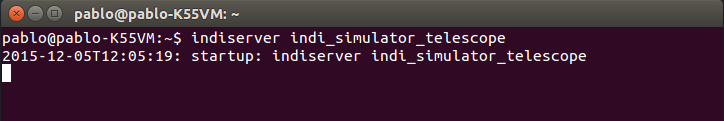
\includegraphics[width=1\textwidth]{./imagenes/capturaINDIServer}
\caption{Lanzamiento del Simulador de Telescopio} \label{fig:INDIServer}
\end{figure}

\section{Lanzando el Prototipo de Cliente}
Una vez que está lanzado el simulador con el que vamos a trabajar, tenemos que abrir el fichero principal denominado \textit{parser.html}.

En el momento que tengamos abierto el fichero \textit{parser.html} en el navegador, se nos solicitará una IP y un puerto válido que corresponderá con un servidor INDI\ref{fig:conexionINDI}.\\

Al conectar con el servidor, nos aparecerá una ventana correspondiente al dispositivo que estamos simulando. Por el contrario, si no se ha lanzado ningún simulador, al conectar con el servidor se mostrarán los diferentes dispositivos conectados con el servidor en ese momento. \\

Cada dispositivo se muestra en una ventana y a partir de ahí se puede interaccionar con él realizando todas las modificaciones que se quieran, analizando los datos que se obtienen, etc.
\begin{figure}[htb]
\centering
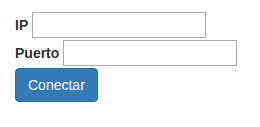
\includegraphics[width=0.7\textwidth]{./imagenes/capturaConexion}
\caption{Conexión con el Servidor INDI} \label{fig:conexionINDI}
\end{figure}

\section{Encender un Dispositivo}
Cuando se ha realizado la conexión con el servidor y hemos lanzado algún simulador hay que tener en cuenta que, por regla general, el dispositivo estará apagado. Su pantalla principal tendrá un desplegable para realizar la función de conexión. Además de ese desplegable, es posible que tenga una pestaña que pertenezca a un grupo, que será el de Opciones, con el nombre del dispositivo, su versión y algunos datos referentes al dispositivo. \\

Una vez que en la pestaña principal del dispositivo se inicia la conexión, se muestran todos los grupos de Propiedades y sus correspondientes y específicas propiedades para interactuar con el dispositivo.
\begin{figure}[htb]
\centering
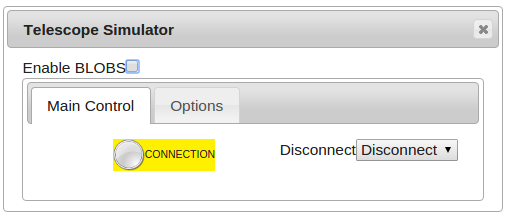
\includegraphics[width=0.9\textwidth]{./imagenes/capturaEncendiendo}
\caption{Encendiendo un Dispositivo} \label{fig:encendiendoDispositivo}
\end{figure}

\section{Interactuar con un Dispositivo}
Cuando se establece la conexión y encendemos el dispositivo, tenemos acceso a toda su información  que está agrupada en diferentes grupos podemos decir que ya estamos conectados con el dispositivo\ref{fig:capturaDispositivo}.\\

Hay que tener bien claro que las propiedades se pueden o no modificar, dependiendo del tipo de permiso que tengan. Las propiedades que se pueden modificar tendrán un desplegable, un cuadro de texto, un cuadro numérico o un \textit{checkbox}. Además hay que decir, que salvo los desplegables, las demás propiedades tendrán siempre un botón para poder actualizar los diferentes valores y enviarlos así al servidor.
\begin{figure}[htb]
\centering
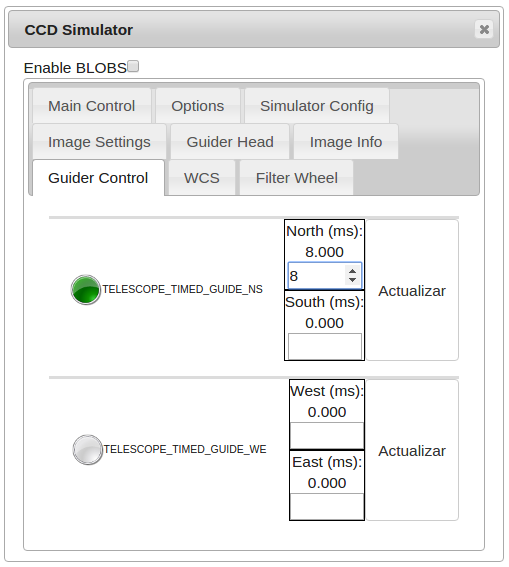
\includegraphics[width=1\textwidth]{./imagenes/capturaDispositivo}
\caption{Dispositivo CCD Encendido} \label{fig:capturaDispositivo}
\end{figure}

\subsection{Estado de una Propiedad}
